
% \course{Information Systems Engineering}
% \matriculationyear{2018}
% \issuedate{29.4.2025}
% \duedate{29.9.2025}
% \professor{Prof. Dr. Wolfgang E. Nagel}
%
%
% \begin{task}[] % If needed, a custom title can be provided between the brackets
% 	\minisec{\objectivesname}\smallskip
% In addition to the performance of computer systems, energy efficiency is another relevant metric for their evaluation. In this thesis, the student analyzes the energy efficiency methods of the Intel Sapphire Rapids architecture and evaluates their effects on performance and power consumption. This includes an assessment of the power-saving mechanisms defined in the ACPI standard, as well as the integrated monitoring methods for power consumption.
%
% 	\minisec{\focusname}\smallskip
% 	\begin{itemize}
% 		\item Background research (processor manuals and source code of low-level applications)
% 		\item Architecture analysis and comparison with other architectures
% 		\item Description of existing power saving methods and benchmarks thereof
% 		\item Analysis of internal measurement interfaces for power-related metrics
% 		\item Definition and execution of the appropriate benchmarks for an evaluation of the impact on performance and power consumption
% 		\item Evaluation and presentation of the results
% 	\end{itemize}
% \end{task}

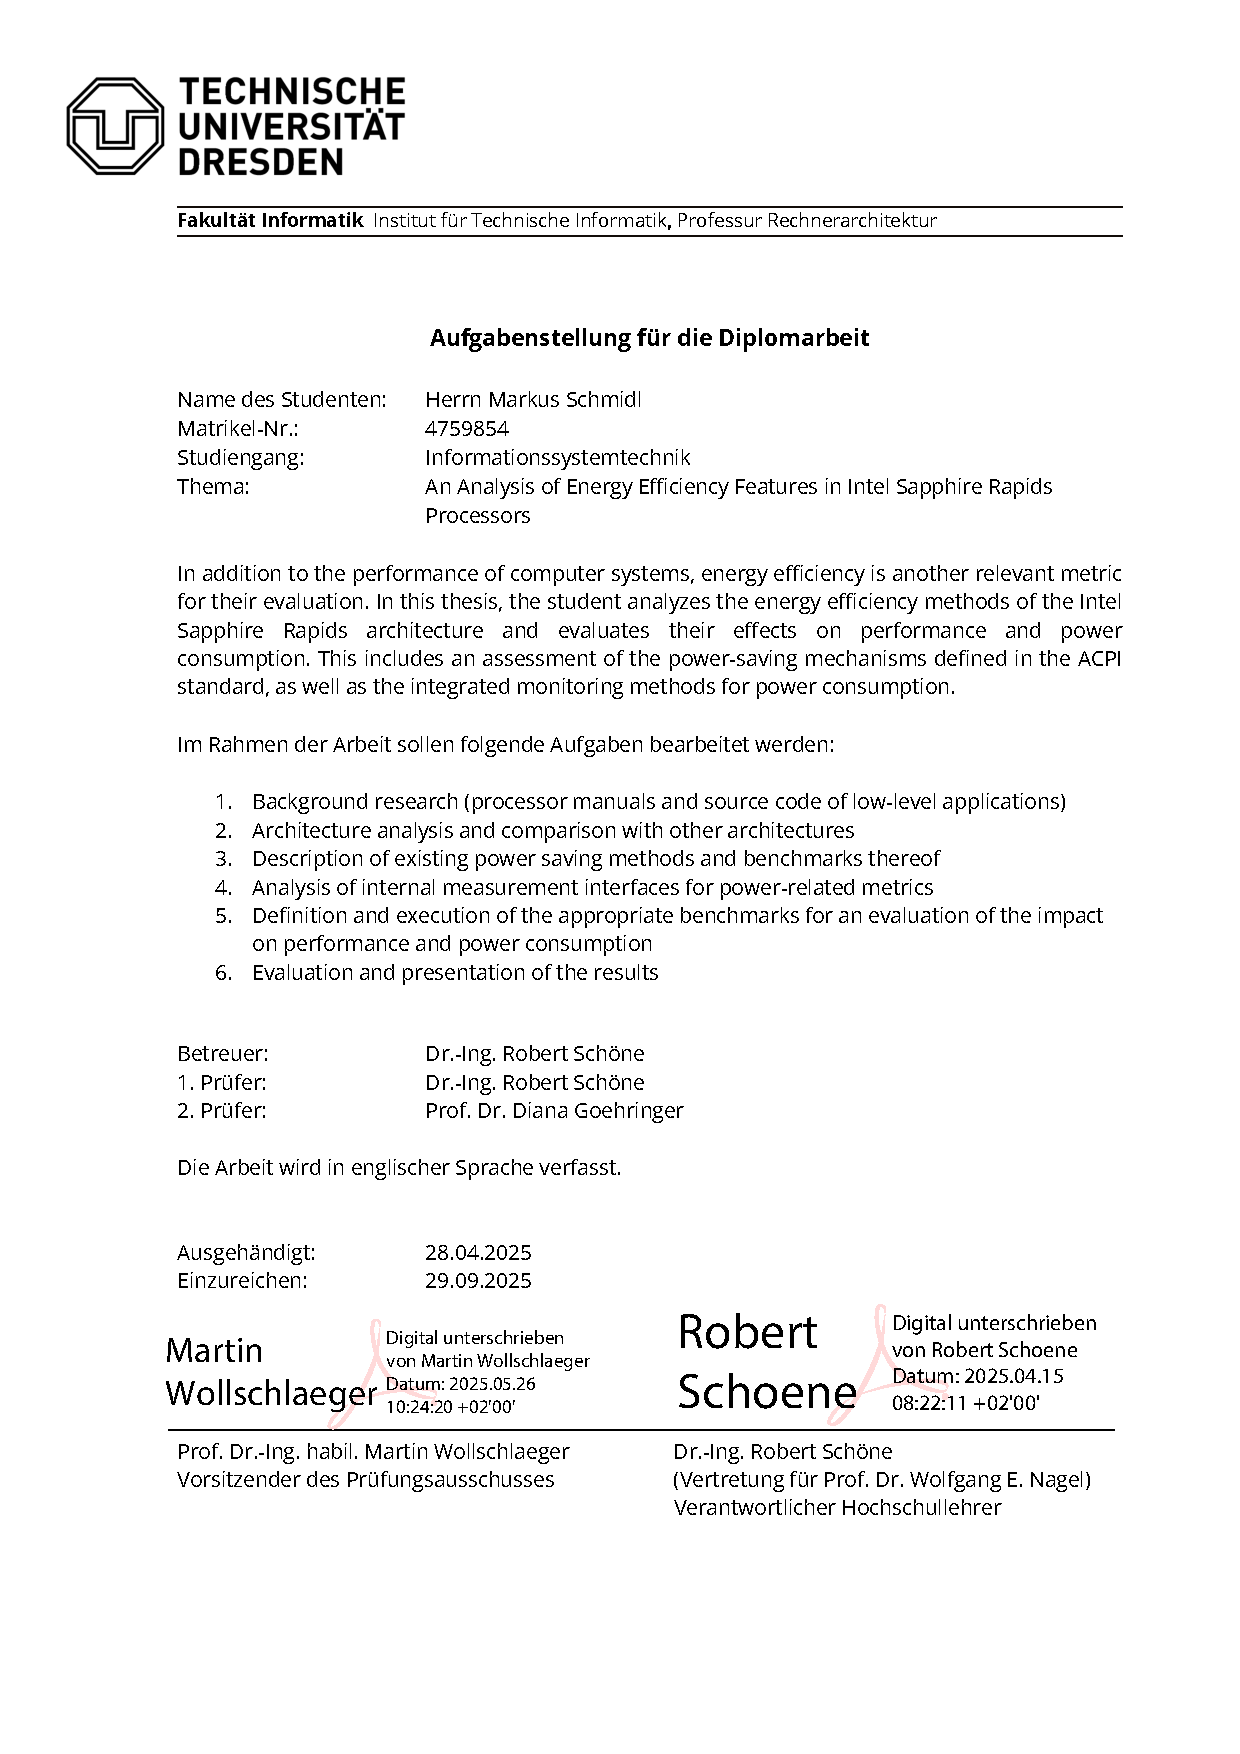
\includepdf[pages=-]{0_frontmatter/task_description.pdf}